\chapter{Introduction}
\label{ch:introduction}
\pagenumbering{arabic}
\pagestyle{headings}

\section{Structure of the document}
%%%TBD

\section{Motivation and description of the problem}
\label{sec:bdotp}
This project aims to simplify and enhance management and monitoring capabilities of network administrators using Bird Daemon  software on top of an OpenWRT/LEDE-based Firmware. This project is a second iteration in the development of an existing configuration integration package already being used by OpenWRT/LEDE's community.

\subsection{Motivation}
\label{sec:motivation}
Back in 2014, while working on my BSc. dissertation in the Universitat Politècnica de Catalunya, the department and, specifically, the investigation team I was working with, gave me the opportunity to participate in a GSoC\footnote{Google Summer of Code (\href{https://www.google-melange.com/archive/gsoc/2014/orgs/freifunk/projects/eloicaso.html}{2014})} project under the umbrella of Freifunk, to design, develop and demonstrate a package that would help simplifying the configuration of Bird Daemon as a software able to share routes between BMX6 mesh and BGP infrastructure networks deployed in \textit{frontier} nodes deployed in the Catalan community network Guifi.net.

That project was successful and the result was an integration package using OpenWRT's well-known UCI/LUCI configuration mechanism to set up Bird through a user-friendly Web UI even without deep knowledge of Bird's syntax. GSoC's time frame though was not enough to polish the package and add some secondary protocols and the package stopped getting maintenance from myself later that year. However, it has been an OSS project that has been on my \textit{backlog} of things I want to keep improving and also been queried some times by Víctor Oncins as it is really helpful for network administrators but it is not mature enough for complex production environments available in Guifi.net.

Therefore, I have been really fortunate to have the opportunity to retake this package as my MSc. project while doing my MSc. and work together with Víctor as this has meant that I have had direct feedback from administrators using the tool in production environments and to improve its most critical features. Moreover, Víctor has also published a report on GitHub \cite{bgpbmx6} describing the main challenges found using the old version of the Package and a deep description of the environment.

\subsection{Bird Daemon}
Bird Daemon\footnote{Bird Daemon: \href{http://bird.network.cz/}{Link}} (from now onwards Bird) is an open source Internet Routing service (daemon) that allows network administrators to simplify route sharing configuration, management and monitoring of different routing protocols by using Routing tables as \textit{transferable} knowledge and a powerful filtering c-like language to achieve it with really fine-grained results. Bird manages its own configuration also following a c-like scheme and this was the main goal of my 2014 project: to automate and simplify it by using UCI instead and letting the Package do the translation to Bird configuration.

Bird current version is 1.6.3 and its functionality is split in two different Daemons, one for IPv4 (Bird4) and one for IPv6 (Bird6). This version supports the following routing protocols:

\subsubsection{Routing Protocols}
\begin{itemize}
    \item \textbf{\href{https://www.irif.fr/~jch//software/babel/}{Babel}}: IGP\footnote{Interior Gateway Protocol: routing protocols being used in internal Autonomous Systems to manage their connectivity and paths.}\footnote{Autonomous System: Single-administrated network behaving as an entity.} distance-vector protocol stated as being in alpha stage of adoption.
    This protocol is not available to automate through our Package yet.
    \item \textbf{Open Shortest Path First - OSPF}: IGP link-state protocol fully supported for both IPv4 \href{https://tools.ietf.org/html/rfc2328}{OSPFv2} and IPv6 \href{https://tools.ietf.org/html/rfc5340}{OSPFv3}.
    This protocol has some functionality available for IPv4 in the Package but is not fully functional and there is no UI supporting it. OSPF support is one of the top priorities for future Package improvements.
    \item \textbf{\href{https://www.rfc-editor.org/rfc/rfc2453.txt}{Routing Information Protocol - RIP}}: IGP distance-vector protocol fully supported. This protocol is completely deprecated by other distance-vector protocols as OSPF, which are less constrained by network's scale.
    This protocol is not available to automate through our Package and, because it is obsolete, there are not plans to implement it in short term.
    \item \textbf{\href{https://www.rfc-editor.org/rfc/rfc4271.txt}{Border Gateway Protocol - BGP}}: EGP\footnote{Exterior Gateway Protocol: routing protocols managing connectivity and paths on networks compound by Autonomous System entities.} path-vector protocol fully supported. This is the most common protocol for backbone networks and the key protocol for this project.
    This protocol is available to automate through the Package but only the most common or relevant options have been implemented. BGP's support finalisation is one of the top priorities for future Package improvements. 
\end{itemize}.

\subsubsection{Support Protocols}
\label{sub:sub:supproto}
The following list of \textit{Protocols} are not exactly routing protocols but supportive implementations of different capabilities or services to enhance and simplify system's management.

\begin{itemize}
    \item \textbf{Static}: Bird's mechanism to implement \textit{smart} static routes. It allows  origin or pattern discrimination and modification. For example, configure any route in 10.0.0.0/16 to be unreachable or to extend it with an attribute: \texttt{ospf\_metric = 100}.
    Static Protocol is available to automate through the Package.
    \item \textbf{Pipe}: Routing Tables are the main knowledge units for Bird (e.g BGP \& OSPF primary tables). Pipe Protocol allows to connect different Routing Tables and to apply discrimination to the routes the share (e.g BGP->OSPF accept all and OSPF->BGP accept if part of 10.0.0.0/8).
    Pipe Protocol is available to automate through the Package.
    \item \textbf{Direct}: Route generator for any targeted interface. Bird uses pattern matching to include/exclude any network interface that we want to be encapsulated as a single bunch of \textit{device} routes.
    Direct Protocol is available to automate through the Package.
    \item \textbf{Device}: This \textit{protocol} is required in most of the Bird configurations and its main purpose is to gather key data from system's interfaces in order to facilitate Bird's operation.
    Device Protocol is available to automate through the Package.
    \item \textbf{Kernel}: Bird's implementation to allow sharing routes between the Operative System Kernel Routing Tables and the ones designated by Bird.
    Kernel Protocol is available to automate through the Package. There are plans to improve this protocol as there is one process left to be automated through UI and it is top priority.
    \item \textbf{RAdv}: Implementation of the Router Advertisement Protocol (\href{https://tools.ietf.org/html/rfc4861}{IPV6's Neighbour Discovery}) allowing a fine-grained control of how often the neighbour discovery information is sent and which information is shared on them per target.
    RAdv Protocol is not available to automate through the Package. There are not plans to implement it in short term.
    \item \textbf{\href{https://www.rfc-editor.org/rfc/rfc5880.txt}{Biderectional Forwarding Detection - BFD}}: This \textit{protocol} is a standalone tool for neighbours monitoring in order to foresee some protocol service disruptions by monitoring peers in a more efficient way than most protocols do. This protocol consists in a session created by real routing protocols (e.g OSPF and BGP) and its sole role is to notify them in case of an event. This protocol is almost fully supported (except of verbose mode and authentication).
    BFD Protocol is not available to automate through the Package. There are not plans to implement it in short term.
\end{itemize}

\subsection{OpenWRT/LEDE's configuration integration package}
Bird-OpenWrt Package (from now onwards \textit{the Package}) is an open source OpenWRT/LEDE-specific solution (\textit{.ipk}) integrated by four separated packages (two for Bird IPv4 (\textit{bird4-uci}) and IPv6 (\textit{bird6-uci}) UCI integration and the other two for Web UI management (\textit{luci-app-bird4} and \textit{luci-app-bird6}) providing Bird Daemon a user-friendly configuration scheme (UCI) and a graphical interface in OpenWRT/LEDE-based routers. All the implementation details are covered in chapter \ref{ch:implementation}.

\subsection{Bird Daemon administration issues}
\label{subsec:bdai}
As part of the GSoC project, the solution provided was not mature enough to fulfil all the requirements:
\begin{itemize}
    \item Tight time-frame forcing to prioritise the key capabilities to implement.
    \item Some key protocols were not enabled in the final solution because they were not relevant for GSoC's scope (e.g Pipe or Direct).
    \item Some secondary protocols were not enabled in the final solution because they were not relevant for GSoC's scope (e.g OSPF or Babel).
    \item Some basic processes require manual (terminal) changes.
    \item No possible way to edit Filters or Functions files through Web UI.
    \item No Bird Daemon Status feedback (e.g no way to know if bird is running or failed to start through Web UI).
    \item No possible way to see Bird Daemon's Log information through Web UI.
    \item Bird's API changed (from Bird 1.4.3 to 1.6.3) making bird crash using base Package configuration.
    \item No possible way of monitoring Bird's current status (e.g full information for BGP connections).
\end{itemize}
\section{Scope of the project}
\label{sec:sotp}
This project's scope is to adopt as many of the mentioned enhancements that are clearly aligned with eradicating required manual changes in command line, improve the UX\footnote{UX: User eXperience} and to align the packet with current Bird Daemon API in the given time frame of 3 months. As a result of a \textit{backlog} prioritization, the following items were agreed (in priority order):

\begin{itemize}
    \item Update the package to the latest Bird API.
    \item Update old version's disruptive issues (e.g disabled Protocols).
    \item Status, Log, Filters and Functions Graphical integration.
    \item Theoretical viability investigation of uBus integration.
\end{itemize}


\subsection{Deviations from the original plan and future  work}
While agreeing the original scope of the project, few extra ideas and tasks were planned but, as a matter of priorities and time constraints, some were dismissed or set as future work.

\begin{itemize}
    \item Add secondary protocols: adopt more key features from Bird and increasing the range of administrators being able to take advantage of this Package.
    \item Integrate next generation of Web UI using LUCI2: HTML/JavaScript-based UI instead of LUA-based.
    \item Implementation of uBus integration according to the results of the investigation done in this project.
    \item Comparative set of tests between Quagga and Bird Daemon solutions.
\end{itemize}

Most of these extra tasks are already documented as part of the Package Documentation Reporitory\footnote{GitHub TODO List: \href{https://github.com/eloicaso/bgp-bmx6-bird-docn/blob/master/EN/TODO.md}{Link}.} and open for discussion and Pull Requests\footnote{Pull Request: Changes pushed to a repository by an external party (e.g a fork repository pushing changes to its parent.} to add extra requirements.

\subsubsection{Bird Daemon Vs. Quagga deployments}
There is a special reasoning behind not doing a comparative analysis of these two solutions. Of course, the timing constrains have strongly influenced the decision of dropping this comparison from this project's scope, but there is also the big amount of evidence already collected for my GSoC2014 project as well as some new evidence found either in some reputable sources as well as from Bird's own OSS Community proving that Bird Daemon has been far more stable, less resource eater and flexible (thanks to its Filter\&Function scripting language) than other well-known enterprise level solutions. This evidence and where it is coming from is available in the Appendix \ref{app:ch:blinks}.


\subsection{Methodology and communication}
This project starts with the premise that there is no need for a wide initial investigation phase as the Package used was designed and developed by myself. Nevertheless, there are three foreseen introductory tasks:
\begin{itemize}
    \item Refresh the Package to the latest Bird Daemon version API. 
    \item Investigate, understand and document the production environment.
    \item Update Documentation and prepare the repositories required (documentation, package and dissertation).
\end{itemize}

After this initial phase, the implementation tasks will be executed in a Kanban-like approach:
\begin{itemize}
    \item Features will be executed following Backlog's priority order and one at a time.
    \item Each \textit{feature} or \textit{requirement} must be self-contained and the Package should be releasable at any time.
    \item There is no Board or framework to introduce the data (e.g time spent or state of the tasks) as such as the overhead of doing it is not proportional to the number of tasks or value of the data that could be collected. However, during the first \textit{Cycle} of the project (first two weeks), in order to illustrate how could this project look like using Kanban, I did use an online OSS tool called \textit{Taiga.io}\footnote{\href{https://taiga.io/}{Taiga.io}: Online project management tool working either with Kanban or SCRUM Agile methodologies. This tool is widely used in OSS projects due to its power, simplicity and plugins (open API) and has also enterprise options.}. See Appendix \ref{app:sec:kanban} in order to see some captures of the initial tasks created using the tool.
    \item There will be weekly/bi-weekly meetings with the Stakeholder in order to discuss progress, any blocker or issue and rearrange priorities if required.
    \item There will be a \textit{demo} to the Stakeholder to show progress in a weekly/bi-weekly basis.
\end{itemize}

The communication, as already mentioned, will be done through regular meetings with the External Consultant (Stakeholder) using the Jitsi\footnote{\href{https://jitsi.org/}{Jitsi}: Open Source multiplatform VoIP conference service.} conference service, which allows screen sharing and text communication while in conference, simplifying demoing and code reviews. Regular communication will be also done through Hangouts instant messaging service and by email to share progress, risks or blockers.

\subsubsection{Gantt Diagram}
Tasks' delivery forecast can be seen in Figures  \ref{fig:general_gantt} and \ref{fig:detail_gantt}:

\begin{landscape}

\begin{figure}[h!]
\centering
    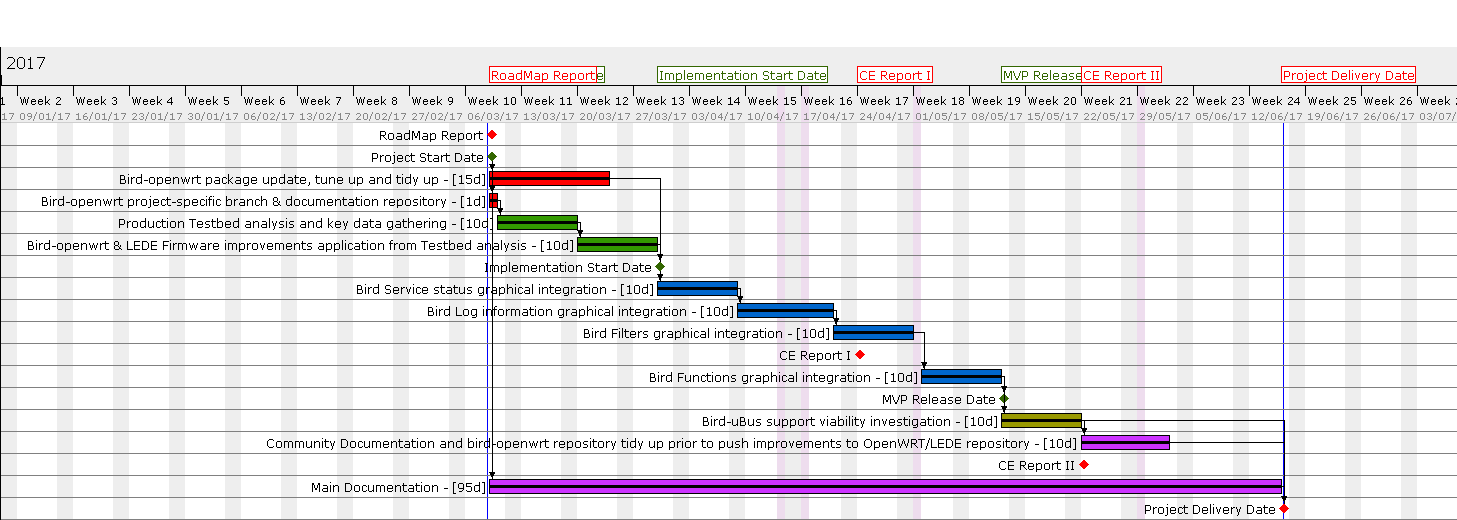
\includegraphics[width=\hsize]{images/gantt}
    \caption{Tasks schedule}
    \label{fig:general_gantt}
\end{figure}

Key milestones:
\begin{itemize}
    \item \textbf{Project's start date \& RoadMap Report} (09/03/17): initial Package refresh and production environment investigation. Project's goals formal report and when they are expected to be delivered.
    \item \textbf{Project's implementation start date} (30/03/17): beginning of features' implementation.
    \item \textbf{Continuous Evaluation Report I} (22/04/17): formal report to present Project's progress, pending work, any issue or blocker and updated  timeline.
    \item \textbf{MVP Release} (12/05/2017): forecast delivery date of the final version of the Package. No extra changes planned unless the investigation task requires them.
    \item \textbf{CE Report II} (22/05/17): optional progress report prior to Project's delivery.
    \item \textbf{Project Delivery Date} (12/06/17): final date to deliver the dissertation, slides, recording and any extra archive required.
\end{itemize} 

\begin{figure}[h!]
    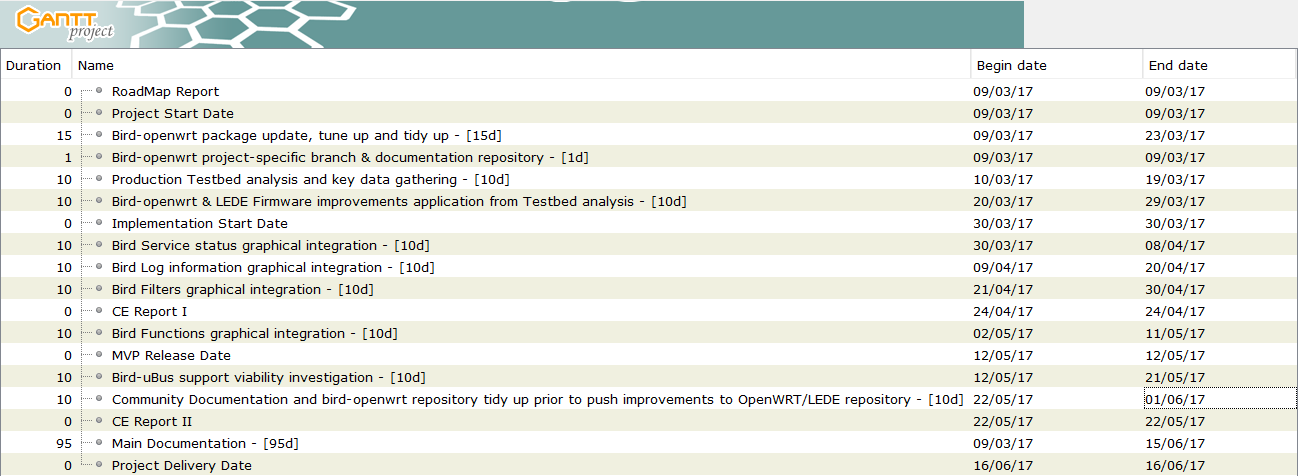
\includegraphics[width=\hsize]{images/gantt_data}
    \caption{Schedule details}
    \label{fig:detail_gantt}
\end{figure}
\end{landscape}


\section{Background information}
\label{sec:backc}
\subsection{Guifi.net}
\label{subsec:gn}
Guifi.net is a community network working for and by its own users (self-organised) giving an affordable alternative for anyone willing to connect to the Internet. This network's principles are freedom; open design, administration and management; and neutrality. This network was born in Catalonia as a wireless network but it has spread all over the world with about 33.124\footnote{Guifi.net live statistics: \href{https://guifi.net/guifi/menu/stats/nodes}{Link}} active nodes (as 26/05/17) using roof antennas and optical fiber deployments.

This network is connected to the Catalan Internet Exchange Point (CATNIX\footnote{CATNIX: \href{http://www.catnix.net/en/}{Link}}), it has its own Government Foundation\footnote{Fundació Guifi.net: \href{https://fundacio.guifi.net/Foundation}{Link}} to promote and protect network's principles defined in an operational and behavioural common regulation (Comuns - XOLN\footnote{\href{https://guifi.net/en/FONNC}{XOLN/FONN}: Compact for a Free, Open \& Neutral Network}). Any company that adheres adheres to the XOLN/FONNC principles will be able to professionally operate and advertise itself as a Guifi.net Internet or other services provider.

Finally, although Guifi.net main routing protocol is BGP for infrastructure and OSPF for internal routing, there are several isles\footnote{Guifi.net Mesh Networks: \href{http://ca.wiki.guifi.net/wiki/Annex:subxarxes_mesh}{Link}}\footnote{\href{http://qmp.party/Documentation}{qMp}: Most commonly used firmware in Guifi.net for mesh networks. This OpenWRT fork aims to simplify and automate mesh deployments.} operating as Mesh Networks using BMX6 dynamic routing protocol.

\subsection{OpenWRT/LEDE Project}
\label{subsec:owrtlp}
OpenWRT, and its Fork LEDE-Project\footnote{LEDE-Project: Linux Embedded Development Environment.}, are Open Source Linux-based firmwares primarily focused on commodity routers, but aiming to work in any Linux-based system. This firmware supports a wide variety of manufacturer's hardware and also a wide range of software, services and routing protocols to enhance, secure and efficiently operate as a standalone router and service provider.

\subsection{Infrastructure vs Mesh Network Routing Protocols}
\label{subsec:dsrp}
Routing protocols' job is to receive a route and, according to its attributes and the information stored in the system, to redirect this route to the next step towards its destination or to drop it. However, each protocol follows different principles in order to achieve the best performance using different algorithms or paradigms. Moreover, depending on who is consuming the network and which are its requirements, we could prioritise either scalability, stability or resilience and prioritise how much critical are the previous characteristics for our consumers:

\begin{itemize}
    \item \textbf{Infrastructure Networks}: commonly used in \textit{backbone} networks. Stable, robust and highly scalable. Their main handicap is that it suffers from big overheads on topology changes (e.g low/non fault tolerance) and that it has big convergence times in large-scale networks.
    \item \textbf{Mesh Networks}: oppositely to classic dynamic networks, mesh networks' strength is to be able to converge almost instantly after any topology event. These networks work in a cooperative manner in order to achieve a fully connected network (point-to-multipoint) where all the nodes share network's knowledge in order to optimise routes and nodes floods the network in order to keep network's topology knowledge up to date.
\end{itemize}

\subsubsection{BGP}
\label{subsubsec:bgp}
BGP is a dynamic infrastructure IP routing protocol designed for large-scale internet topologies (EGP\footnote{EGP: Exterior Gateway Protocol. This includes all the protocols that routes between Autonomous systems.}). Its routing algorithm relies on the best path according to route's attributes.

\subsubsection{BMX6}
\label{subsec:bmx6}
Batman-eXperimental6 \cite{bmx6} is a fork of the Mesh protocol BATMAN\footnote{\href{https://www.open-mesh.org/projects/open-mesh/wiki}{B.A.T.M.A.N}: Better Approach To Mobile Adhoc Networking.}. This is a mesh networking routing protocol is compatible with most of linux-like systems but only operates with IPv6 networks. This routing protocol uses a table-driven\footnote{Table-driven: Compose a routing table with all the source-destination entries.} distance-vector approach\footnote{Distance-vector: Best path (cost of going) from source to destination.}.

\subsubsection{UCI}
The Unified Configuration Interface (\href{https://wiki.openwrt.org/doc/uci}{UCI}) aims to centralise OpenWrt's packages and system configuration. This mechanism is widely used for almost, if not all, the packages working in OpenWrt. UCI allows you to easily, and in a human-readable manner, simplify administration overheads.

\subsubsection{LUCI}
LUCI is OpenWrt's solution to graphically represent and allow UCI settings' configuration via web pages (UI is generated on Server-side). It uses Lua\footnote{\href{https://www.lua.org/manual/5.1/}{Lua}: open source powerful language optimised for embedded environments.} language following the MVC\footnote{MVC: Model View Controller Software architecture pattern. This is \textbf{just one} of the different patterns of logically separate a program's \textit{intelligence} between data, logic and UI avoiding tangled \textit{spaghetti code}.} software pattern.

%and a modelling parser called CBI\footnote{\href{https://github.com/openwrt/luci/wiki/CBI}{CBI}: Lua model parser UCI-to-HTML.}.
LUCI's components are:
\begin{itemize}
    \item CBI (Model): CBI files include UCI definitions and \textit{describe} HTML's final form (e.g optional/mandatory properties, order of apparition, and all the required logic to validate entered data through the forms.
    \item Controller: Web pages definition (e.g data or rendering target) and communication functions required by the Model (CBI) page.
    \item View: HTML templates defining how a page, section or specific element is represented.
\end{itemize}

\subsubsection{LUCI2}
\label{sub:sub:luci2}
LUCI2\footnote{\href{https://wiki.openwrt.org/doc/techref/luci2}{LUCI2}: 2nd generation of OpenWrt UCI UI modeling architecture. This second version uses HTML/CSS/JavaScript and communication through JSON messages instead of Lua.} is the next version of LUCI using client-side web technologies to enhance and simplify UI creation, releasing these router's resources. Moreover, this new version uses standard communication process between browser and http server (JavaScript's XHR\footnote{XMLHttpRequest(\href{https://xhr.spec.whatwg.org/}{XHR}): standard communication mechanism to transfer objects embedding them in the URL but avoiding page reloads. Most common object's format in OpenWrt/LEDE is JSON.}) using the RPC Daemon\footnote{\href{https://wiki.openwrt.org/doc/techref/rpcd}{Remote Procedure Calls}: Client-Server communication mechanism for network systems (router).} and uBus Daemon\footnote{\href{https://wiki.openwrt.org/doc/techref/ubus}{Universal Bus} (uBus): is a daemon providing a \textit{space} for packages or protocols to register their APIs allowing external access to it acting as a pipe between them. uBus use RPC calls through the RPC Daemon available in OpenWrt.} as query brokers between UI's Front End, Server's Back End and router's internal Daemons providing services under RPCd.

This new version is not completely defined and it has been evolving together with OpenWrt/LEDE and LUCI. There is no much documentation of its definition, API, how to use it or integration examples and, therefore, it is complex to get the full picture of how it works and how to start using it and it is common to see packages using both CBIs(LUCI) and HTML/CSS/JS(LUCI2) approaches together according to the complexity or level of customisation required to represent the data.

The already mentioned lack of documentation in LUCI2 will be repeated during section \ref{sec:luciimp} as it was a critical handicap while implementing some UI pages with \textit{simple} data structures, but requiring some customisation and process automation, which LUCI2 solves efficiently if you know how to do it.
